%%%%%python description starts
\section{Python}
\label{sec:python-start}
Python is a general-purpose, high-level, remarkably powerful dynamic programming language 
that is used in a wide variety of application domains. Its high-level built-in data structures, 
combined with dynamic typing and dynamic binding, make it very attractive for Rapid Application Development, 
as well as for use as a scripting or glue language to connect existing components together. 
Python's simple, easy to learn syntax emphasizes readability and therefore reduces the cost of program maintenance. 
Python supports modules and packages, which encourages program modularity and code reuse. 
The Python interpreter and the extensive standard library are available in source or binary form without 
charge for all major platforms, and can be freely distributed \cite{python-ref}.


\subsection{Downloading and installing on Windows} \label{py-windows}
This book uses Python 3 for demonstrating the experiments, both on Windows 
and Linux. Since Python uses indentation to indicate a block of code, 
the users are advised to install a programmer text editor like Atom. 
This editor will allow the readers to modify the Python scripts on their 
machines if they want to. Starting from download, we shall go through the 
steps to set up Python 3 on Windows OS:

\begin{enumerate}
      \item Visit the URL {\tt https://www.python.org/}. 
      At the top of the page, locate the Downloads tab and click on it. 
      At the time of writing this book, Python 3.9.4 
      is the latest version. Click on Download Python 3.9.4 to download the 
      executable file. The readers may want to download the other versions of 
      Python 3. However, we recommend the installation of Python 3.5 or above. 
      It may be noted that some of the Python 3 versions cannot be used on Windows 7 or earlier.
      \item Locate the executable file and double-click on it to begin the 
      installation. Python 3.9.4 Setup window appears, as shown in \figref{python-windows}. 
      In this window, check the box which says, Add Python 3.9 to PATH and 
      click on Install now.  
      \begin{figure}
            \centering
            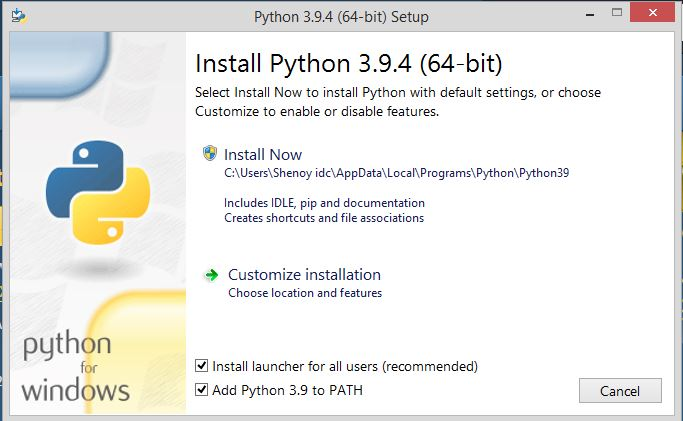
\includegraphics[width=\lgfig]{\LocSWfig/python-windows-install.JPG}
            \caption{Installing Python 3 on Windows}
            \label{python-windows}
      \end{figure}
\end{enumerate}

Once the installation is finished, Python 3.9 App can be launched 
from the Start menu. In this book, we will use the Command Prompt to 
execute the Python scripts. Please note that a Python script has .py as its 
extension. Carry out the steps given below to execute a Python script from 
the Command Prompt:

\begin{enumerate}
      \item Launch the Command Prompt. Press the Windows key+R together. 
      A window, as shown in \figref{windows-run} appears. In the text box adjacent to {\tt Open}, type {\tt cmd}, 
      and press Enter. The Command Prompt, as shown in \figref{windows-cmd} appears. 
      By default, it points to the home directory.  
      \begin{figure}
            \centering
            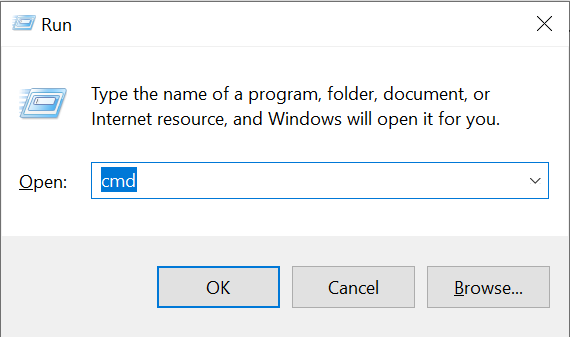
\includegraphics[width=\lgfig]{\LocSWfig/windows-cmd.png}
            \caption{Launching the Command Prompt on Windows}
            \label{windows-run}
      \end{figure}
      \item Now, we will check whether Python 3.9 was installed 
      successfully or not. In the Command Prompt, type {\tt py -{}-version} and 
      press Enter. If this step displays Python 3.9.4 in the following line, 
      the installation was successful. 
      \begin{figure}
            \centering
            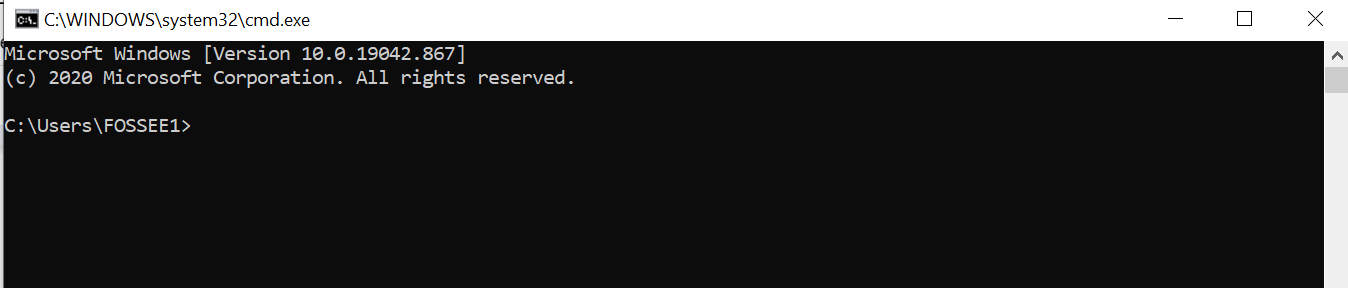
\includegraphics[width=\lgfig]{\LocSWfig/win-command-prompt.png}
            \caption{Command Prompt on Windows}
            \label{windows-cmd}
      \end{figure}
      \item Using the {\tt cd} command, navigate to the directory where your Python 
      script is located. Assuming that your Command Prompt points to the 
      home directory, and you want to navigate to the folder Origin on 
      Desktop, execute the following command: {\tt cd Desktop\textbackslash Origin} \\
      It may be noted that a backslash (\textbackslash) has been used between 
      Desktop and Origin. 
      \item To view the contents of this folder, type {\tt dir} and press Enter.
      \item Suppose you have a Python script named  {\tt FILENAME.py} in this 
      folder. To execute this script, type {\tt python FILENAME.py} and press 
      Enter. The required output will be displayed in the Command Prompt itself. 
      We don’t expect the readers to run the command {\tt python FILENAME.py} at 
      this instant. This command will be helpful while running the Python 
      scripts in the upcoming sections and chapters. 
      \item To exit the Command Prompt, type {\tt exit} and press Enter. 
 
\end{enumerate}

Apart from Python, we need to install Python Serial Port Extension, 
also known as pyserial \cite{pySerial}. To do so, carry out the steps given 
below:
\begin{enumerate}
      \item Launch the Command Prompt, as shown in \figref{windows-run}. 
      \item First, we need to make sure we have pip available. 
      In the Command Prompt, execute the following command: {\tt py -m pip -{}-version} \\ 
      This step should display an output with the version of pip installed. 
      \item Now, install pyserial. In the Command Prompt, execute the following command: 
      {\tt py -m pip install pyserial}  
      \item We will verify whether the pyserial package was installed successfully or not. 
      In the Command Prompt, execute the following command: 
      {\tt pip show pyserial}
      It should show the name, version, etc., of the package. 
      \item To exit the Command Prompt, type {\tt exit} and press Enter. 
\end{enumerate}

\subsection{Downloading and installing on GNU/Linux Ubuntu} \label{py-linux}
On Linux, we can install Python from the terminal. Please ensure that you 
are connected to the Internet. To install Python 3.5, carry out the steps given below:
\begin{enumerate}
      \item Open a terminal by pressing the Alt+Ctrl+T keys together.
      \item Update the system by executing the command {\tt sudo apt-get update}
      \item Install Python3.5 by executing the command given below:\\
      {\tt sudo apt-get install python3.5}
      \item Now, we will check whether Python was installed 
      successfully or not. In the terminal, type {\tt python3 -{}-version} or type {\tt python3 -V}  and 
      press Enter. If this step displays Python 3.8.4 in the following line, 
      the installation was successful. 
\end{enumerate}

Once the installation is finished, Python 3 can be launched 
from the terminal. In this book, we will use the Linux terminal to 
execute the Python scripts. Please note that a Python script has .py as its 
extension. Carry out the steps given below to execute a Python script from 
the terminal:
\begin{enumerate}
      \item Open a terminal by pressing the Alt+Ctrl+T keys together.
      \item Using {\tt cd} command, navigate to the directory where the Python script is located. 
      \item Suppose you have a Python script named  {\tt FILENAME.py}. 
      To execute this script, type {\tt python3 FILENAME.py} and press 
      Enter. The required output will be displayed in the terminal itself. 
      We don’t expect the readers to run the command {\tt python3 FILENAME.py} at 
      this instant. This command will be helpful while running the Python 
      scripts in the upcoming sections and chapters. 
\end{enumerate}

Apart from Python, we need to install Python Serial Port Extension, 
also known as pyserial \cite{pySerial}. To do so, carry out the steps given 
below:
\begin{enumerate}
      \item Open a terminal by pressing the Alt+Ctrl+T keys together.
      \item First, we need to install pip. In the terminal, execute the following command: 
      {\tt sudo apt-get install python3-pip} 
      \item Now, install pyserial. In the terminal, execute the following command:\\ 
      {\tt pip3 install pyserial}  
      \item We will verify whether the pyserial package was installed successfully or not. 
      In the terminal, execute the following command: 
      {\tt pip3 show pyserial}\\
      It should show the name, version, etc., of the package. 
\end{enumerate}

% \begin{enumerate}
%       \item On Ubuntu, Python can be installed from the command line by typing in the
%             following commands:

%             \$ sudo apt-get install python3.5 \\
%             This will install python 3.5 as this set of tools are compatible with python3. It also
%             works all other versions of python3.  
%             \$ pip3 install python-serial \\
%             This will install serial package required for communicating with Arduino Uno.
%       \item 1. On Windows,


%             Download Windows python compiler Self Extracting Archive (.exe)  (32-bit or 64-bit as per your system) from https://www.python.org/downloads/windows/

%             Download Windows pyserial package .exe from https://pypi.python.org/pypi/pyserial/3.4.
%             After downloading run the .exe file and follow the instructions.

%             Now that we have Python installed, open the terminal by typing 'Ctrl+Alt+T'.
%             Enter the command 'python'. This opens the Python REPL (Read Eval Print Loop).
%             Python files have .py extension and .py files can be executed by typing "python3 filename.py"
%             on the python terminal. Please visit the link https://github.com/manasdas17/Python3-Arduino for 
%             the library. 

% \end{enumerate}

\subsection{Python-Arduino toolbox}
\label{sec:python-toolbox}
Python, by default, does not have the capability to connect to Arduino. 
All such add-on functionalities are added to Python using packages. 
Python-Arduino toolbox can be found inside the {\tt Origin/tools/python} directory, 
see \fnrefp{fn:file-loc}.  This toolbox is compatible for both of the operating systems: Windows and Linux. 
The Python scripts (or codes) for various experiments mentioned throughout this book can be found in 
{\tt Origin/user-code} directory. The {\tt user-code} directory will have many sub-directories as per the experiments. 

In this book, we have created a package named "Arduino" in Python 3.  This package is available at 
{\tt Origin/tools/python}. This package makes use of the functions available in pyserial \cite{pySerial} to 
establish serial communication with Arduino. In this package, we have added functions required to run 
various experiments on \arduino. Using this basic set of functions, the user can define other functions to operate
upon the Arduino. Please note that the "Arduino" package and the FLOSS firmware  given 
in \ardref{ard:firmware} are required to run the experiments. 

Now, we will see how to import (or load) the "Arduino" package inside a Python script to run 
various experiments provided in this book. In a Python script, add {\tt from Arduino.Arduino import Arduino} 
at the top of the script. When we add {\tt from Arduino.Arduino import Arduino} in a script, the function "from" 
searches for "Arduino" only in that directory where our script is saved. That's why all the scripts in Python 
must be saved in a folder that contains the "Arduino" package. In this book, "Arduino" package has been saved 
in the folder where the Python scripts for each chapter are available. For the sake of convenience, we have 
added {\tt from Arduino.Arduino import Arduino} in all the Python scripts provided in this book. 
To run a particular experiment, one can follow the steps as given in \secref{py-windows} or \secref{py-linux}. 


\subsection{Firmware}
\lstset{style=mystyle}
\label{sec:test-firmware-python}
\addtocontents{pyd}{\protect\addvspace{\codclr}}
We have provided a Python code to check whether the firmware has been properly installed. That code is listed below.  
Please ensure that you have uploaded the FLOSS firmware given in \ardref{ard:firmware} on the \arduino\ board.

\begin{pycode}
      \pcaption{A Python script to check whether the firmware is properly installed
            or not}{A Python script to check whether the firmware is properly installed
            or not.  Available at 
            \LocFIMpybrief{test\_firmware.py}. 
            Execute this script by following the steps given in \secref{py-windows} or \secref{py-linux}. If the execution is
            successful, you should expect three "ok" messages.}
      \label{py:test-firmware}
      \lstinputlisting{\LocFIMpycode/test_firmware.py}
\end{pycode}
